\documentclass{article}
\usepackage{enumerate}
\usepackage{amsmath}
\usepackage{amssymb}
\usepackage{graphicx}
\usepackage{subfigure}
\usepackage{geometry}
\usepackage{caption}
\usepackage{indentfirst}
\usepackage{array}
%\renewcommand\arraystretch{2}
\usepackage{tikz}
\usepackage{multicol}
\usepackage{algorithm}  
\usepackage{algorithmicx}  
\usepackage{algpseudocode}
\renewcommand{\algorithmicrequire}{\textbf{Input:}}  
\renewcommand{\algorithmicensure}{\textbf{Output:}}  

\geometry{left=3.0cm,right=3.0cm,top=3.0cm,bottom=4.0cm}
\renewcommand{\thesection}{Ex. \arabic{section}}
\title{VE281 Writing Assignment Three}
\author{Liu Yihao 515370910207}
\date{}

\begin{document}
\maketitle

\section{}
Let $u_i$ be the number of elements in the $i^{th}$ slot of the hash table generated by the hash function $h$, then 
$$|U|=\sum\limits_{i=0}^{n-1}u_i$$
$$|U|^2=\left(\sum\limits_{i=0}^{n-1}u_i\right)^2=\sum\limits_{i=0}^{n-1}u_i^2+2\sum_{i=0}^{n-2}\sum_{j=i+1}^{n-1}u_iu_j< n\sum\limits_{i=0}^{n-1}u_i^2$$
$$\epsilon\geqslant Pr(h(k)=h(l))=\frac{\sum\limits_{i=0}^{n-1}u_i(u_i-1)}{|U|^2}=\frac{\sum\limits_{i=0}^{n-1}u_i^2-|U|}{|U|^2}>\frac{\dfrac{|U|^2}{n}-|U|}{|U|^2}=\frac{1}{n}-\frac{1}{|U|}$$
$$\epsilon>\frac{1}{n}-\frac{1}{|U|}$$

\section{}
From the lecture, we know the $H$ as set of all functions that map from $U$ to $\{0,1,2,\dots,n-1\}$ is universal, so $$\mathop{Pr}\limits_{h\in H}(h(k)=h(l))\leqslant\frac{1}{n}$$

Now, we can take away $n$ functions that map $U$ to $\{0\},\{1\},\dots,\{n-1\}$ from $H$ to form $H'$, since these function always collide for all $k\neq l$, taking away them can decrease the average probability of collision. Then we can find that $$\mathop{Pr}\limits_{h\in H'}(h(k)=h(l))<\frac{1}{n}$$

Here is a simple example:

Let $n=2$, $|U|=3$, $H=\{h_i(x)|x\in U,i=0,1,2,3,4,5\}$, define $h_i(x)$ as following table:
\begin{center}
\begin{tabular}{|c|c|c|c|c|c|c|}
\hline
$x$ & $h_0(x)$ & $h_1(x)$ & $h_2(x)$ & $h_3(x)$ & $h_4(x)$ & $h_5(x)$ \\\hline
0 & 1 & 0 & 0 & 1 & 1 & 0\\\hline
1 & 0 & 1 & 0 & 1 & 0 & 1\\\hline
2 & 0 & 0 & 1 & 0 & 1 & 1\\\hline
\end{tabular}
\end{center}
$$Pr(h(0)=h(1))=Pr(h(1)=h(2))=Pr(h(0)=h(2))=\frac{1}{3}<\frac{1}{2}$$
\section{}
$$U(L)=\frac{1}{2}\left[1+\left(\frac{1}{1-L}\right)^2\right]\leqslant8.5\Longrightarrow L\leqslant 0.75$$
$$S(L)=\frac{1}{2}\left(1+\frac{1}{1-L}\right)\leqslant3\Longrightarrow L\leqslant0.8$$

So $L=0.75$ should be chosen, the hash table size should be $600/0.75=800$.

\section{}
We want to prove that if the number of full nodes is $n$, then  the number of leaves in a non-empty binary tree is $n+1$. Mathematical induction is used to prove it.

First, when $n=0$, there is no full node, so the number of leaves is obviously 1.

Then, when $n=k$, suppose the statement is true. When $n=k+1$, one more full node is added now. We know each node have three status: full node, not full node and leaf. We can't add more nodes to a full node. When we add a node to a not full node, it becomes a full node, and there is one more leaf. When we add a node to a leaf, the leaf becomes a not full node, so the number of leaves doesn't change. So we can concluded that when $n=k+1$, the number of leaves is $k+2$, the statement is proved.

\section{}
\begin{enumerate}[(a)]
\item A$\to$B$\to$C$\to$D$\to$E$\to$F$\to$G$\to$H$\to$I
\item D$\to$C$\to$F$\to$G$\to$E$\to$B$\to$I$\to$H$\to$A
\item C$\to$D$\to$B$\to$F$\to$E$\to$G$\to$A$\to$I$\to$H
\item A$\to$B$\to$H$\to$C$\to$E$\to$I$\to$D$\to$F$\to$G
\end{enumerate}

\section{}
\begin{algorithm}[H]
    \begin{algorithmic}
        \Require The root node $root$
        \State push $root$ into $stack$
        \While {$stack$ is not empty}
            \State $node\gets$ pop a element from $stack$
            \If {$node.right$ exists}
            	\State push $node.right$ into $stack$
            \EndIf
            \If {$node.left$ exists}
            	\State push $node.left$ into $stack$
            \EndIf
            \State do something with $node$
        \EndWhile
    \end{algorithmic}  
\end{algorithm}

\section{}
\begin{enumerate}[(a)]
\item \ 
\begin{center}
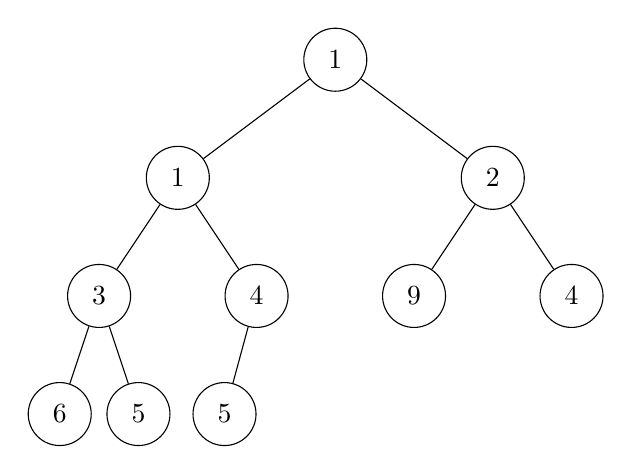
\begin{tikzpicture}
\tikzstyle{every node}=[draw,shape=circle,minimum size=0.8cm];
\node {1}[sibling distance=4cm]
child { node {1}[sibling distance=2cm]
	child {
		node {3}[sibling distance=1cm]
		child { node {6} }
		child { node {5} }
	}
	child {
		node {4}[sibling distance=1cm]
		child[left] { node {5} }
	}
}
child { node {2}[sibling distance=2cm]
	child {
		node {9}[sibling distance=1cm]
	}
	child {
		node {4}[sibling distance=1cm]
	}
};
\end{tikzpicture}
\end{center}
\item \ 
\begin{center}
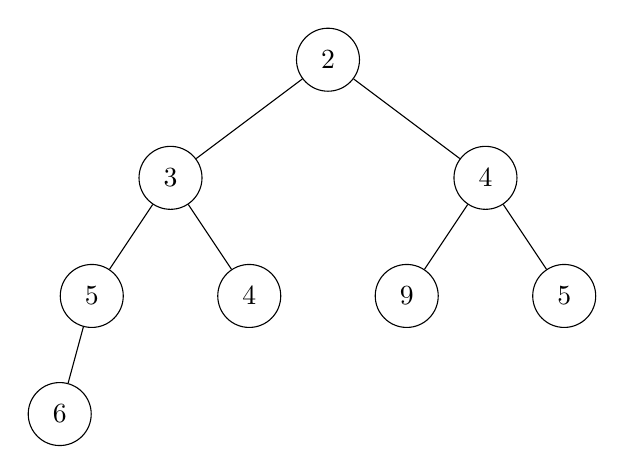
\begin{tikzpicture}
\tikzstyle{every node}=[draw,shape=circle,minimum size=0.8cm];
\node {2}[sibling distance=4cm]
child { node {3}[sibling distance=2cm]
	child {
		node {5}[sibling distance=1cm]
		child[left] { node {6} }
	}
	child {
		node {4}[sibling distance=1cm]
	}
}
child { node {4}[sibling distance=2cm]
	child {
		node {9}[sibling distance=1cm]
	}
	child {
		node {5}[sibling distance=1cm]
	}
};
\end{tikzpicture}
\end{center}
\end{enumerate}

\section{}
\begin{multicols}{2}
\begin{enumerate}
\item 
\begin{center}
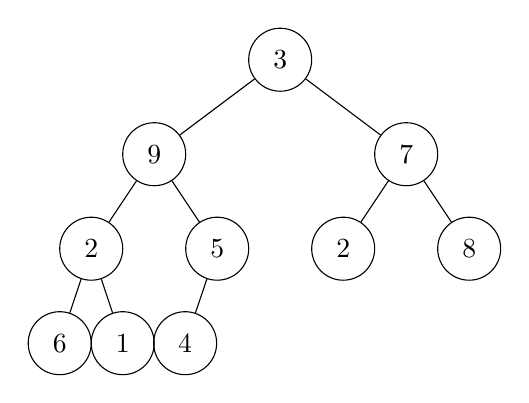
\begin{tikzpicture}[scale=0.8]
\tikzstyle{every node}=[draw,shape=circle,minimum size=0.8cm];
\node {3}[sibling distance=4cm]
child { node {9}[sibling distance=2cm]
	child {
		node {2}[sibling distance=1cm]
		child { node {6} }
		child { node {1} }
	}
	child {
		node {5}[sibling distance=1cm]
		child[left] { node {4} }
	}
}
child { node {7}[sibling distance=2cm]
	child {
		node {2}[sibling distance=1cm]
	}
	child {
		node {8}[sibling distance=1cm]
	}
};
\end{tikzpicture}
\end{center}
\item 
\begin{center}
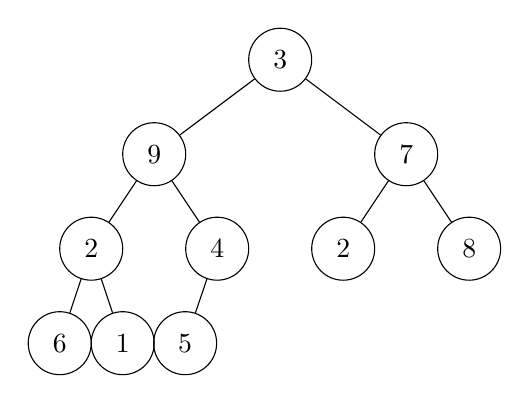
\begin{tikzpicture}[scale=0.8]
\tikzstyle{every node}=[draw,shape=circle,minimum size=0.8cm];
\node {3}[sibling distance=4cm]
child { node {9}[sibling distance=2cm]
	child {
		node {2}[sibling distance=1cm]
		child { node {6} }
		child { node {1} }
	}
	child {
		node {4}[sibling distance=1cm]
		child[left] { node {5} }
	}
}
child { node {7}[sibling distance=2cm]
	child {
		node {2}[sibling distance=1cm]
	}
	child {
		node {8}[sibling distance=1cm]
	}
};
\end{tikzpicture}
\end{center}
\item 
\begin{center}
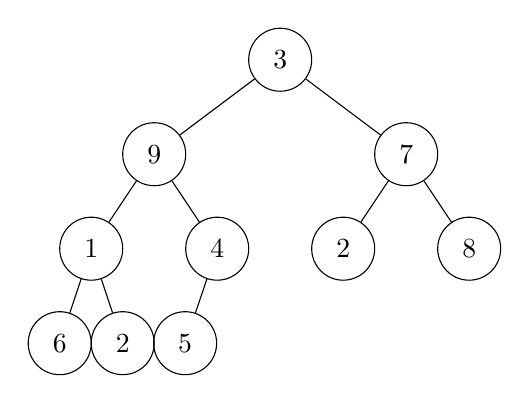
\begin{tikzpicture}[scale=0.8]
\tikzstyle{every node}=[draw,shape=circle,minimum size=0.8cm];
\node {3}[sibling distance=4cm]
child { node {9}[sibling distance=2cm]
	child {
		node {1}[sibling distance=1cm]
		child { node {6} }
		child { node {2} }
	}
	child {
		node {4}[sibling distance=1cm]
		child[left] { node {5} }
	}
}
child { node {7}[sibling distance=2cm]
	child {
		node {2}[sibling distance=1cm]
	}
	child {
		node {8}[sibling distance=1cm]
	}
};
\end{tikzpicture}
\end{center}
\item 
\begin{center}
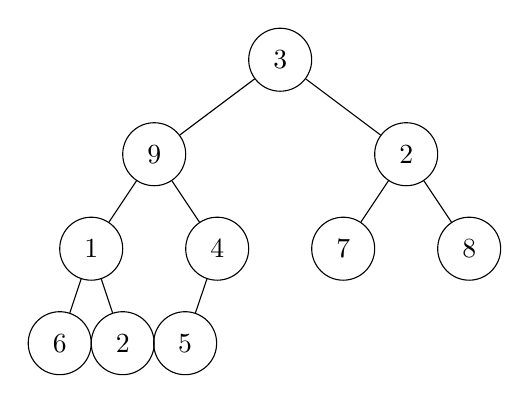
\begin{tikzpicture}[scale=0.8]
\tikzstyle{every node}=[draw,shape=circle,minimum size=0.8cm];
\node {3}[sibling distance=4cm]
child { node {9}[sibling distance=2cm]
	child {
		node {1}[sibling distance=1cm]
		child { node {6} }
		child { node {2} }
	}
	child {
		node {4}[sibling distance=1cm]
		child[left] { node {5} }
	}
}
child { node {2}[sibling distance=2cm]
	child {
		node {7}[sibling distance=1cm]
	}
	child {
		node {8}[sibling distance=1cm]
	}
};
\end{tikzpicture}
\end{center}
\item 
\begin{center}
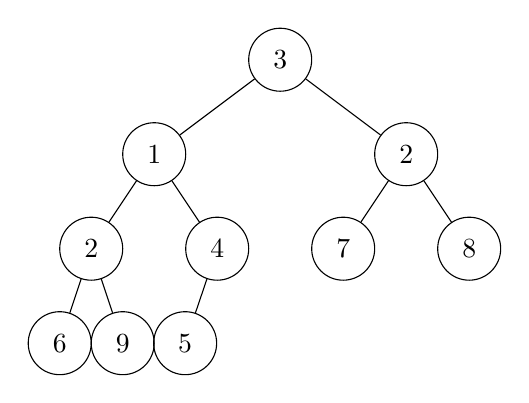
\begin{tikzpicture}[scale=0.8]
\tikzstyle{every node}=[draw,shape=circle,minimum size=0.8cm];
\node {3}[sibling distance=4cm]
child { node {1}[sibling distance=2cm]
	child {
		node {2}[sibling distance=1cm]
		child { node {6} }
		child { node {9} }
	}
	child {
		node {4}[sibling distance=1cm]
		child[left] { node {5} }
	}
}
child { node {2}[sibling distance=2cm]
	child {
		node {7}[sibling distance=1cm]
	}
	child {
		node {8}[sibling distance=1cm]
	}
};
\end{tikzpicture}
\end{center}
\item 
\begin{center}
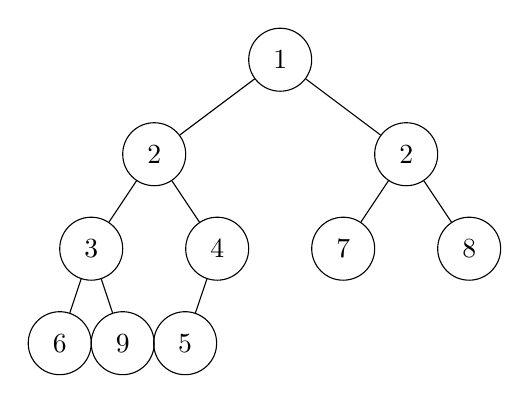
\begin{tikzpicture}[scale=0.8]
\tikzstyle{every node}=[draw,shape=circle,minimum size=0.8cm];
\node {1}[sibling distance=4cm]
child { node {2}[sibling distance=2cm]
	child {
		node {3}[sibling distance=1cm]
		child { node {6} }
		child { node {9} }
	}
	child {
		node {4}[sibling distance=1cm]
		child[left] { node {5} }
	}
}
child { node {2}[sibling distance=2cm]
	child {
		node {7}[sibling distance=1cm]
	}
	child {
		node {8}[sibling distance=1cm]
	}
};
\end{tikzpicture}
\end{center}
\end{enumerate}
\end{multicols}

\end{document}
